\documentclass[12pt,utf8,notheorems,compress,t,aspectratio=169]{beamer}
\usepackage{etex}

\usepackage{pgfpages}
\usepackage[export]{adjustbox}

% Workaround for the issue described at
% https://tex.stackexchange.com/questions/164406/beamer-using-href-in-notes.
\newcommand{\fixedhref}[2]{\makebox[0pt][l]{\hspace*{\paperwidth}\href{#1}{#2}}\href{#1}{#2}}

\usepackage[english]{babel}

\usepackage{mathtools}
\usepackage{xspace}
\usepackage{booktabs}
\usepackage{stmaryrd}
\usepackage{amssymb}
\usepackage{manfnt}
\usepackage{array}
\usepackage{ragged2e}
\usepackage{multicol}
\usepackage{tabto}
\usepackage{xstring}
\usepackage{proof}
\usepackage{agda}
\usepackage[all]{xy}
\xyoption{rotate}
\usepackage{tikz}
\usetikzlibrary{calc,shapes,shapes.callouts,shapes.arrows,patterns,fit,backgrounds,decorations.pathmorphing,positioning,svg.path}
\hypersetup{colorlinks=true}

\DeclareFontFamily{U}{bbm}{}
\DeclareFontShape{U}{bbm}{m}{n}
   {  <5> <6> <7> <8> <9> <10> <12> gen * bbm
      <10.95> bbm10%
      <14.4>  bbm12%
      <17.28><20.74><24.88> bbm17}{}
\DeclareFontShape{U}{bbm}{m}{sl}
   {  <5> <6> <7> bbmsl8%
      <8> <9> <10> <12> gen * bbmsl
      <10.95> bbmsl10%
      <14.4> <17.28> <20.74> <24.88> bbmsl12}{}
\DeclareFontShape{U}{bbm}{bx}{n}
   {  <5> <6> <7> <8> <9> <10> <12> gen * bbmbx
      <10.95> bbmbx10%
      <14.4> <17.28> <20.74> <24.88> bbmbx12}{}
\DeclareFontShape{U}{bbm}{bx}{sl}
   {  <5> <6> <7> <8> <9> <10> <10.95> <12> <14.4> <17.28>%
      <20.74> <24.88> bbmbxsl10}{}
\DeclareFontShape{U}{bbm}{b}{n}
   {  <5> <6> <7> <8> <9> <10> <10.95> <12> <14.4> <17.28>%
      <20.74> <24.88> bbmb10}{}
\DeclareMathAlphabet{\mathbbm}{U}{bbm}{m}{n}
\SetMathAlphabet\mathbbm{bold}{U}{bbm}{bx}{n}

\usepackage{pifont}
\newcommand{\cmark}{\ding{51}}
\newcommand{\xmark}{\ding{55}}
\DeclareSymbolFont{extraup}{U}{zavm}{m}{n}
\DeclareMathSymbol{\varheart}{\mathalpha}{extraup}{86}

\graphicspath{{images/}}

\usepackage[protrusion=true,expansion=true]{microtype}

\setlength\parskip{\medskipamount}
\setlength\parindent{0pt}

\title{Modal operators for a constructive account of well quasi-orders}

\author{Ingo Blechschmidt}
\date{November 30th, 2024}

\setbeameroption{show notes on second screen=bottom}
\newcommand{\jnote}[2]{\only<#1>{\note{\setlength\parskip{\medskipamount}\footnotesize\justifying#2\par}}}

%\useinnertheme[shadow=true]
\setbeamerfont{block title}{size={}}

\useinnertheme{rectangles}

\usecolortheme{orchid}
\usecolortheme{seahorse}
\definecolor{mypurple}{RGB}{253,73,34}
\definecolor{mypurpledark}{RGB}{100,0,150}
\setbeamercolor{structure}{fg=mypurple}
\setbeamercolor*{title}{bg=mypurple,fg=white}
\setbeamercolor*{titlelike}{bg=mypurple,fg=white}
\setbeamercolor{frame}{bg=black}

\usefonttheme{serif}
\usepackage[T1]{fontenc}
\usepackage{libertine}

% lifted from https://arxiv.org/abs/1506.08870
\DeclareFontFamily{U}{min}{}
\DeclareFontShape{U}{min}{m}{n}{<-> udmj30}{}
\newcommand\yon{\!\text{\usefont{U}{min}{m}{n}\symbol{'210}}\!}

\newcommand{\A}{\mathcal{A}}
\newcommand{\B}{\mathcal{B}}
\newcommand{\C}{\mathcal{C}}
\newcommand{\M}{\mathcal{M}}
\renewcommand{\AA}{\mathbb{A}}
\newcommand{\BB}{\mathbb{B}}
\newcommand{\pp}{\mathbbm{p}}
\newcommand{\MM}{\mathbb{M}}
\newcommand{\E}{\mathcal{E}}
\newcommand{\F}{\mathcal{F}}
\newcommand{\FF}{\mathbb{F}}
\newcommand{\G}{\mathcal{G}}
\newcommand{\J}{\mathcal{J}}
\newcommand{\GG}{\mathbb{G}}
\renewcommand{\O}{\mathcal{O}}
\newcommand{\K}{\mathcal{K}}
\newcommand{\NN}{\mathbb{N}}
\newcommand{\QQ}{\mathbb{Q}}
\newcommand{\RR}{\mathbb{R}}
\newcommand{\TT}{\mathbb{T}}
\newcommand{\PP}{\mathbb{P}}
\newcommand{\ZZ}{\mathbb{Z}}
\newcommand{\CC}{\mathbb{C}}
\renewcommand{\P}{\mathcal{P}}
\newcommand{\aaa}{\mathfrak{a}}
\newcommand{\bbb}{\mathfrak{b}}
\newcommand{\ccc}{\mathfrak{c}}
\newcommand{\ppp}{\mathfrak{p}}
\newcommand{\fff}{\mathfrak{f}}
\newcommand{\mmm}{\mathfrak{m}}
\newcommand{\defeq}{\vcentcolon=}
\newcommand{\defeqv}{\vcentcolon\equiv}
\newcommand{\Cov}{\mathrm{Cov}}
\renewcommand{\_}{\mathpunct{.}}
\newcommand{\?}{\,{:}\,}
\newcommand{\speak}[1]{\ulcorner\text{\textnormal{#1}}\urcorner}
\newcommand{\inv}{inv.\@}
\newcommand{\forces}{\vDash}
\newcommand{\ind}{\ensuremath{_\text{ind}}\xspace}
\newcommand{\sinf}{\ensuremath{_\infty}}
\newcommand{\impl}{\ensuremath{_\text{impl}}\xspace}

\setbeamertemplate{blocks}[shadow=false]

\newenvironment{indentblock}{%
  \list{}{\leftmargin\leftmargin}%
  \item\relax
}{%
  \endlist
}

% Adapted from https://latex.org/forum/viewtopic.php?t=2251 (Stefan Kottwitz)
\newenvironment<>{hilblock}{
  \begin{center}
    \begin{minipage}{9.05cm}
      \setlength{\textwidth}{9.05cm}
      \begin{actionenv}#1
        \def\insertblocktitle{}
        \par
        \usebeamertemplate{block begin}}{
        \par
        \usebeamertemplate{block end}
      \end{actionenv}
    \end{minipage}
  \end{center}}

\newenvironment{changemargin}[2]{%
  \begin{list}{}{%
    \setlength{\topsep}{0pt}%
    \setlength{\leftmargin}{#1}%
    \setlength{\rightmargin}{#2}%
    \setlength{\listparindent}{\parindent}%
    \setlength{\itemindent}{\parindent}%
    \setlength{\parsep}{\parskip}%
  }%
  \item[]}{\end{list}}

\tikzset{
  invisible/.style={opacity=0,text opacity=0},
  visible on/.style={alt={#1{}{invisible}}},
  alt/.code args={<#1>#2#3}{%
    \alt<#1>{\pgfkeysalso{#2}}{\pgfkeysalso{#3}}}
}

% https://tex.stackexchange.com/questions/172336/drawing-roman-laurel-leaves-spqr-in-tikz
\tikzset{
  laurel-wreath/.pic = {
    \fill svg{M14.4-24.6c-1.5-1.5-2.6-3.3-3.1-5.3l-.4-1.7c-.2-1.1-.2-4.1 .2-5.7 .2-.9 .3-1.3 .5-1.3l1.4 1.1 2.5 2.4c2.7 2.5 5.2 6 5.8 8 .2 .6-.5 .3-2.2-.9-1.6-1.3-3.3-2.6-5-3.8l.1 1.4c.2 1.4 .5 2.7 1.1 4.6s.8 2.5 .5 2.5l-1.4-1.3zm69.6 1.1 .3-1.2c.8-2.3 1.3-4.8 1.6-7.3l-1.5 1.1c-1.3 .9-2.6 1.9-3.7 3-1.6 1.1-2 1.3-2.1 1 .7-1.8 1.6-3.4 2.8-4.9 1.3-1.7 6.5-6.8 7-6.8 .2 0 .3 .2 .3 .5l.3 1.6c.3 2.2 .2 5.7-.5 7.4-.8 1.9-1.6 3.1-3 4.7-1.1 1.1-1.4 1.3-1.5 .9z};
    \fill svg{M10-29.4c-.8-1.1-1.4-2.2-2-4.1l-.7-3.5c-.2-3 .2-4.4 1.4-8.3l.5-1.4c.2-1.3 .3-1.9 .6-1.9 .3-.2 .6 .3 .7 .8s.9 2.2 1.9 3.6c1.4 2.2 2.7 4.4 3.9 6.6l.9 2.7c0 .6 0 .6-.3 .6-.6 0-4.9-4.4-5.8-6l-.2-.6-.1 1.7-.3 2.8c-.3 2.7-.3 3.8 0 5.5 .6 2 .5 2.4-.5 1.5zm79.2 .3 .4-2.4c.2-1.3 .2-2.7-.1-4.9l-.3-2.8v-1.6l-.7 1c-.8 1.3-5 5.5-5.5 5.5s-.5-.3 .2-1.9c.5-1.7 1.4-3.3 3.3-6.5 2.4-3.6 2.7-3.9 2.8-4.7 .5-1.3 .5-1.4 .8-1.2 .3 0 .6 .8 .6 1.5l.7 2.4c.9 2.7 1.1 3.6 1.2 6 .2 3.1-.5 6-2 8.2-.8 1.3-1.3 1.7-1.4 1.5z};
    \fill svg{M5-40c-.4-3.2-.1-6.5 .9-9.6 .5-1.1 1.6-2.8 2.2-3.4l1.3-1.6 2-2.7 .2 .6c.1 1.3 .4 2.6 .9 3.8l.3 1c.8 1.7 1.1 2.7 1.6 5.3 .6 2.5 .6 4.6 .2 4.6-.3 0-.9-.8-1-1.1l-.5-.8c-1.4-2-3-5.2-2.9-6.5-.9 2.7-2 5.4-3.5 7.9l-.3 .8-.3 .8c0 .5-.6 1.6-.8 1.6l-.3-.7zm89.2 .2-.2-.5-.3-.9-1.1-2.7-1.1-2.4c-.6-1.4-1.2-2.8-1.6-4.2l-.3 .9c-.3 1.3-1.6 3.9-3 6-1.3 2-1.6 2-1.5 0s1.1-6.3 2.2-9c.8-1.7 1.1-3.1 .9-4.1-.2-1.1 .5-.8 2.2 1.8 3.3 4.4 3.8 5.4 4.4 7.8 .6 2.4 .5 7.7-.3 7.8l-.3-.5z};
    \fill svg{M13.9-50.1c-.5-1.9-.8-3.9-.9-5.8-.2-1.6-.1-3.3 .1-4.9-.3 .8-1.7 2.5-4.2 5.1l-3 4.9-.3 .1c-.3 0-.3-2.2 0-3.3 .8-3 1.4-4.6 2.5-6.1 .9-1.3 1.7-1.9 2.5-2.5 1.1-.6 2.7-1.9 3.5-2.7 .9-.9 1.9-1.4 2.2-1.4v1.1l-.3 6.6c0 6.8 .2 6.3-1 8.9-.5 1.1-.8 1.1-1.1 0zm70.8-.4c-.8-2.2-.8-2.5-.7-6.3-.1-2.7-.1-5.5-.2-8.2-.3-1.6-.3-1.9 .5-1.6l.6 .5c1.4 1.4 3 2.5 3.9 3.1 1.3 .9 1.9 1.6 2.7 2.6l.6 .7 .2 .4 .2 .3c.8 .9 2 4.9 2 6.9 .2 1.9-.2 1.9-.9 .5-.7-1.4-1.5-2.7-2.6-4-1.6-1.5-3-3.2-4.2-5 .4 3 .3 6-.5 9 0 .8-.5 2.2-.8 2.3-.2 0-.5-.3-.8-1.2z};
    \fill svg{M16.4-58.5l.2-1.5 .3-3.7c.2-2.8 .3-3.5 1.1-5.4l.7-1.3-.5 .4-1 .7c-.5 .4-1.1 .8-1.5 1.3l-.5 .3-1.9 1.6c-2.2 1.6-2.7 2-3.9 3.6-.5 .8-1.1 1.3-1.3 1.3-.5 0 0-2.4 1.1-4.7 1.5-3.4 4.3-6 7.7-7.4l1.3-.4 1.9-.4 2-.5c1.4 0 1.4 0 1 1.1-.5 .8-.8 2-1.1 4.2-.3 2.3-1.1 4.5-2.2 6.5l-.4 .6c-.6 1.1-1.3 2.1-2 3.2-.5 .6-.8 .8-1 .5zm66.3-.2c-.8-.9-2.8-4.4-3.5-6.1-.6-1.3-.9-2.5-1.1-3.5-.2-2.1-.7-4.1-1.5-6 0-.3 0-.3 1.2-.3l2.1 .5 1.9 .4 1.2 .4 .6 .1 1 .6c3 1.4 5.7 4.6 6.8 8.5l.7 2.6c-.2 .6-.5 .5-1.4-.7-2.2-2.7-4.8-5-7.7-6.9l-1.7-1.3 .6 1.3c.3 .6 .6 1.2 .8 1.9l.3 2.5 .3 3.9c.3 2.4 .2 2.8-.6};
    \fill svg{M21.6-66.1l.4-1.1 .9-3.2c.3-1.9 1.1-3.3 2.4-4.7l.4-.8-1.2 .2-2.2 .3c-2.7 .3-5.3 1.2-7.7 2.5-.6 .5-1.3 .6-1.3 .3 0-.5 .9-1.9 2-2.9 .8-.9 2-1.9 3.2-2.6l.9-.4 2.2-1c.3-.2 1.3-.3 3.2-.1 3 0 4.1 .2 6.3 .7l1.1 .4c.5 .2 .6 .6 .3 .6-.5 0-1.4 .9-1.9 1.7l-1.2 1.8c-1.7 2.8-2.2 3.5-4.6 5.9l-3 2.7-.2-.3zm53.9-2c-2.7-2.8-3.5-3.8-5.4-6.8-.9-1.6-1.4-2.4-1.9-2.5l-.8-.5c-.3 0-.2-.5 .4-.6l1.1-.4c1.9-.6 3-.8 5.6-.9l3.3 .2c2 .6 3.8 1.5 5.4 2.8 .3 0 1.9 1.6 2.5 2.4l.9 1.8c0 .3-.3 .2-1.9-.6-2.8-1.4-4.4-1.9-7.7-2.2l-2.2-.5c-.9-.2-.9-.2-.6 .2 .6 .5 1.7 2 2.1 2.8l.9 2.5c.3 1.5 .6 3 .9 4.6l-2.6-2.3z};
    \fill svg{M34.1-78.7c-3.4-1.3-6.9-2.1-10.6-2.5-.9 0-1.4 0-2.3 .3-2 .5-2 0 0-1.3l2.8-1.2c1.4-.5 1.9-.5 3.8-.6 3.8-.2 6.1 .3 9.3 1.7l3.6 1.1 2.2 .3c1.3 0 1.7 0 2.7-.3 1.1-.3 2.8-1.1 2.8-1.3l-1.3-.9c-1.9-1.4-3.1-2.7-3.1-3.2l.8-.6c.9-.3 1.3-.2 2 .8 .5 .8 1.1 1.4 2.9 2.7 .2 .3 .3 .2 1.1-.3 .9-.8 2.4-2 2.6-2.7 .5-.6 .9-.8 1.8-.5l.8 .6c0 .5-1.4 1.7-3.2 3.2l-1.3 .9c0 .2 1.7 .9 2.9 1.3 .9 .3 1.4 .3 2.7 .3l2.2-.3c1.7-.4 3.4-1 5-1.7 2-.8 4.4-1.3 7.7-1.1 2 .2 2.5 .2 3.8 .6 .9 .3 2.2 .8 2.8 1.2 2 1.1 2 1.6 .2 1.3-1.6-.3-1.9-.3-4.4 0-2.4 .3-4.7 .8-7 1.6l-1.5 .6c-2.9 .3-5.9 .2-8.8-.3-1.7-.3-3.6-.9-6-2.1l-1.1-.4-1.3 .6c-4.5 2.2-9.6 3-14.6 2.2zm-6.3-9.1c};
  }
}

\newcommand{\pointthis}[3]{%
  \tikz[remember picture,baseline]{
    \node[anchor=base,inner sep=0,outer sep=0] (#2) {#2};
    \node[visible on=#1,overlay,rectangle callout,rounded corners,callout relative pointer={(0.3cm,0.5cm)},fill=blue!20] at ($(#2.north)+(-0.1cm,-1.1cm)$) {#3};
  }%
}

\tikzset{
  invisible/.style={opacity=0,text opacity=0},
  visible on/.style={alt={#1{}{invisible}}},
  alt/.code args={<#1>#2#3}{%
    \alt<#1>{\pgfkeysalso{#2}}{\pgfkeysalso{#3}}}
}

\newcommand{\hcancel}[5]{%
  \tikz[baseline=(tocancel.base)]{
    \node[inner sep=0pt,outer sep=0pt] (tocancel) {#1};
    \draw[red!80, line width=0.4mm] ($(tocancel.south west)+(#2,#3)$) -- ($(tocancel.north east)+(#4,#5)$);
  }%
}

\newcommand{\explain}[7]{%
  \tikz[remember picture,baseline]{
    \node[anchor=base,inner sep=2pt,outer sep=0,fill=#3,rounded corners] (label) {#1};
    \node[anchor=north,visible on=<#2>,overlay,rectangle callout,rounded corners,callout
    relative pointer={(0.0cm,0.5cm)+(0.0cm,#6)},fill=#3] at ($(label.south)+(0,-0.3cm)+(#4,#5)$) {#7};
  }%
}

\newcommand{\explainstub}[2]{%
  \tikz[remember picture,baseline]{
    \node[anchor=base,inner sep=2pt,outer sep=0,fill=#2,rounded corners] (label) {#1};
  }%
}

\newcommand{\squiggly}[1]{%
  \tikz[remember picture,baseline]{
    \node[anchor=base,inner sep=0,outer sep=0] (label) {#1};
    \draw[thick,color=red!80,decoration={snake,amplitude=0.5pt,segment
    length=3pt},decorate] ($(label.south west) + (0,-2pt)$) -- ($(label.south east) + (0,-2pt)$);
  }%
}

% Adapted from https://latex.org/forum/viewtopic.php?t=2251 (Stefan Kottwitz)
\newenvironment<>{varblock}[2]{\begin{varblockextra}{#1}{#2}{}}{\end{varblockextra}}
\newenvironment<>{varblockextra}[3]{
  \begin{center}
    \begin{minipage}{#1}
      \begin{actionenv}#4
        {\centering \hil{#2}\par}
	\def\insertblocktitle{}%\centering #2}
        \def\varblockextraend{#3}
	\usebeamertemplate{block begin}}{
        \par
        \usebeamertemplate{block end}
        \varblockextraend
      \end{actionenv}
    \end{minipage}
  \end{center}}

\setbeamertemplate{headline}{}

\setbeamertemplate{frametitle}{%
  \leavevmode%
  \vskip-1.6em%
  \begin{beamercolorbox}[dp=1ex,center,wd=\paperwidth,ht=2.25ex]{title}%
    \vskip0.5em%
    \bf\insertframetitle
  \end{beamercolorbox}%

  \vskip-0.77em\hspace*{-2em}%
  \textcolor{mypurpledark}{\rule[0em]{1.1\paperwidth}{2.4pt}}

  \vskip-0.4em%
}

\setbeamertemplate{navigation symbols}{}

\newcounter{framenumberpreappendix}
\newcommand{\backupstart}{
  \setcounter{framenumberpreappendix}{\value{framenumber}}
}
\newcommand{\backupend}{
  \addtocounter{framenumberpreappendix}{-\value{framenumber}}
  \addtocounter{framenumber}{\value{framenumberpreappendix}}
}

\newcommand{\insertframeextra}{}
\setbeamertemplate{footline}{%
  \begin{beamercolorbox}[wd=\paperwidth,ht=2.25ex,dp=1ex,right,rightskip=1mm,leftskip=1mm]{}%
    % \inserttitle
    \hfill
    \insertframenumber\insertframeextra\,/\,\inserttotalframenumber
  \end{beamercolorbox}%
  \vskip0pt%
}

\newcommand{\hil}[1]{{\usebeamercolor[fg]{item}{\textbf{#1}}}}
\newcommand{\hill}[1]{{\usebeamercolor[fg]{item}{#1}}}
\newcommand{\bad}[1]{\textcolor{red!90}{\textnormal{#1}}}
\newcommand{\good}[1]{\textcolor{mypurple}{\textnormal{#1}}}

\newcommand{\bignumber}[1]{%
  \renewcommand{\insertenumlabel}{#1}\scalebox{1.2}{\!\usebeamertemplate{enumerate item}\!}
}
\newcommand{\normalnumber}[1]{%
  {\renewcommand{\insertenumlabel}{#1}\!\usebeamertemplate{enumerate item}\!}
}
\newcommand{\bigheart}{
\includegraphics{heart}}

\newcommand{\subhead}[1]{{\centering\textcolor{gray}{\hrulefill}\quad\textnormal{#1}\quad\textcolor{gray}{\hrulefill}\par}}

\newcommand{\badbox}[1]{\colorbox{red!30}{#1}}
\newcommand{\infobox}[1]{\colorbox{yellow!70}{\color{black}#1}}

% taken from JDH "The modal logic of arithmetic potentialism and the universal algorithm"
\DeclareMathOperator{\possible}{\text{\tikz[scale=.6ex/1cm,baseline=-.6ex,rotate=45,line width=.1ex]{\draw (-1,-1) rectangle (1,1);}}}
\DeclareMathOperator{\necessary}{\text{\tikz[scale=.6ex/1cm,baseline=-.6ex,line width=.1ex]{\draw (-1,-1) rectangle (1,1);}}}
\DeclareMathOperator{\xpossible}{\text{\tikz[scale=.6ex/1cm,baseline=-.6ex,rotate=45,line width=.1ex]{\draw (-1,-1) rectangle (1,1); \draw[very thin] (-.6,-.6) rectangle (.6,.6);}}}
\DeclareMathOperator{\xnecessary}{\text{\tikz[scale=.6ex/1cm,baseline=-.6ex,line width=.1ex]{\draw (-1,-1) rectangle (1,1); \draw[very thin] (-.6,-.6) rectangle (.6,.6);}}}

% Taken from Todd Lehman (CC-BY-SA) at https://tex.stackexchange.com/a/44920/32372

\newcommand{\setisprime}[1]{
  % Sets \isprime based on #1.
  \ifnum#1=1 \gdef\isprime{0} \else \gdef\isprime{1} \fi
  \foreach \sip in {2, 3,5,...,#1} {
    \pgfmathparse{\sip*\sip>#1? 1:0}
    \ifthenelse{\pgfmathresult=1}{
      % Early-out if \sip^2 > #1.
      \breakforeach
    }{
      % Otherwise test if \sip divides #1.
      \pgfmathparse{Mod(#1,\sip)==0? 1:0}
      \ifthenelse{\pgfmathresult=1}{
        \gdef\isprime{0}
        \breakforeach
      }{}
    }
  }
}

\newcommand{\setxy}[1]{
  % Sets \x and \y to loction of cell #1.
  \pgfmathtruncatemacro{\x}{Mod(#1-1,\cols)}
  \pgfmathtruncatemacro{\y}{(#1-1) / \cols}
  \pgfmathtruncatemacro{\y}{\cols - 1 - \y}
  \pgfmathparse{2.5*(\x+.5)}\let\x\pgfmathresult
  \pgfmathparse{2.5*(\y+.5)}\let\y\pgfmathresult
}

\newcommand{\numlabel}[2]{
  % Draws label #2 at cell #1.
  \setxy{\n}
  \node[fill=none, text=black] at (\x,\y) {#2};
}

\newcommand{\drawpolygon}[2]{
  % Draws polygon with #2 vertexes at cell #1.
  \setxy{#1}
  \ifthenelse{#2>1}{ % Polygon must have at least 2 sides.
    \ifthenelse{#2<30}{ % Draw polygon if it has a small number of sides.
      \filldraw (\x,\y) +(90:1)
      \foreach \drawi in {1,...,#2} {-- +(\drawi/#2*360+90:1)} -- cycle;
    }{ % Else approximate with circle.
      \filldraw (\x,\y) circle(1);
    }
  }{}
}

\newcommand{\setpolygoncolor}[1]{
  % Sets color based on #1.
  \gdef\polycolor{black}
  \ifnum#1=2\gdef\polycolor{black!50!white}\fi
  \ifnum#1=3\gdef\polycolor{yellow!95!red}\fi
  \ifnum#1=5\gdef\polycolor{yellow!0!red}\fi
  \ifnum#1=7\gdef\polycolor{blue!75!green}\fi
  \ifnum#1=11\gdef\polycolor{blue!70!red}\fi
  \ifnum#1=13\gdef\polycolor{blue!40!red}\fi
  \ifnum#1=17\gdef\polycolor{green!50!blue}\fi
  \ifnum#1=19\gdef\polycolor{green!80!black}\fi
  \ifnum#1=23\gdef\polycolor{green!50!red}\fi
  \ifnum#1=29\gdef\polycolor{yellow!50!black}\fi
  \ifnum#1=31\gdef\polycolor{orange!50!black}\fi
  \ifnum#1=37\gdef\polycolor{red!50!black}\fi
  \ifnum#1=41\gdef\polycolor{purple!50!black}\fi
  \ifnum#1=43\gdef\polycolor{blue!50!black}\fi
  \ifnum#1=47\gdef\polycolor{green!50!black}\fi
  \ifnum#1=53\gdef\polycolor{white!50!black}\fi
  \ifnum#1=59\gdef\polycolor{white!50!black}\fi
  \ifnum#1=61\gdef\polycolor{white!50!black}\fi
  \ifnum#1=67\gdef\polycolor{white!50!black}\fi
}

\newcommand{\sieve}[2]{
  \def\cols{#1}
  \def\rows{#2}
  \begin{tikzpicture}[scale=.5]
  \pgfmathtruncatemacro{\nmax}{\rows * \cols}

  \foreach \n in {1,...,\nmax} {
    \begin{scope}[fill=gray, fill opacity=.05,
                  draw=gray, draw opacity=.10,
                  line width=4]
      \drawpolygon{\n}{\n}
    \end{scope}
    \setisprime{\n}
    \ifthenelse{\isprime=1}{
      \numlabel{\n}{\bf\n}
    }{
      \def\startintensity{.33}
      \def\incrintensity{.10}
      \def\intensity{\startintensity}

      \def\m{\n}
      \pgfmathtruncatemacro{\i}{\m / 2}

      % Divide \m by \i until \m is extinguished.
      % Increment \i each time it does not divide into \m.
      \whiledo{\m>1}{
        \setisprime{\i}
        \pgfmathparse{Mod(\m,\i)==0? 1:0}
        \ifthenelse{\pgfmathresult=1\and\isprime=1}{
          \setpolygoncolor{\i}
          \begin{scope}[fill=\polycolor, fill opacity=\intensity,
                        draw=\polycolor!85!black, draw opacity=\intensity,
                        line width=\intensity*1.5]
            \drawpolygon{\n}{\i}
          \end{scope}
          \pgfmathtruncatemacro{\m}{\m / \i}
          \pgfmathparse{\intensity + \incrintensity}\let\intensity\pgfmathresult
        }{
          \pgfmathtruncatemacro{\i}{\i - 1}
          \def\intensity{\startintensity}
        }
      }
      \begin{scope}[text=black, text opacity=.5]
        \numlabel{\n}{\scriptsize\n}
      \end{scope}
    }
  }

  \end{tikzpicture}
}


\newcommand{\triang}{\hil{$\blacktriangleright$}}
\newcommand{\concat}{\mathbin{{+}\mspace{-8mu}{+}}}

\newcommand{\astikznode}[2]{\tikz[baseline,remember picture]{\node[anchor=base,inner sep=0,outer sep=0.1em] (#1) {#2};}}
\newcommand{\astikznodecircled}[3]{\tikz[baseline,remember picture]{\node[anchor=base,circle,draw=#2,thick,inner sep=0.05em,outer sep=0.05em] (#1) {#3};}}
\newcommand{\astikznodetransparentlycircled}[2]{\tikz[baseline,remember picture]{\node[anchor=base,circle,opacity=0,draw=white,text opacity=1,thick,inner sep=0.05em,outer sep=0.05em] (#1) {#2};}}

\setbeamersize{text margin left=1.60em,text margin right=1.60em}

\newlength\stextwidth
\newcommand\makesamewidth[3][c]{%
  \settowidth{\stextwidth}{#2}%
  \makebox[\stextwidth][#1]{#3}%
}

\newcommand{\dnote}[1]{%
  \begin{tabular}{@{}m{2em}@{}m{0.83\textwidth}@{}}%
    \textdbend &#1%
  \end{tabular}%
  \par
}

\newcommand{\genalpha}{\mbox{$\hspace{0.12em}\shortmid\hspace{-0.62em}\alpha$}}

\usepackage{newunicodechar}

\newunicodechar{∇}{\ensuremath{\nabla}}
\newunicodechar{λ}{\ensuremath{\lambda}}
\newunicodechar{σ}{\ensuremath{\sigma}}
\newunicodechar{τ}{\ensuremath{\tau}}
\newunicodechar{∷}{\ensuremath{\!\!\!}}
\newunicodechar{⧺}{\ensuremath{\!\!\!}}
\newunicodechar{₁}{\ensuremath{_1}}
\newunicodechar{₂}{\ensuremath{_2}}
\newunicodechar{∈}{\ensuremath{\in}}

\begin{document}

\addtocounter{framenumber}{-1}

\definecolor{mypurpleblack}{RGB}{30,0,50}
\setbeamercolor{structure}{fg=black}

{\usebackgroundtemplate{\begin{minipage}{\paperwidth}\centering\vspace*{-7em}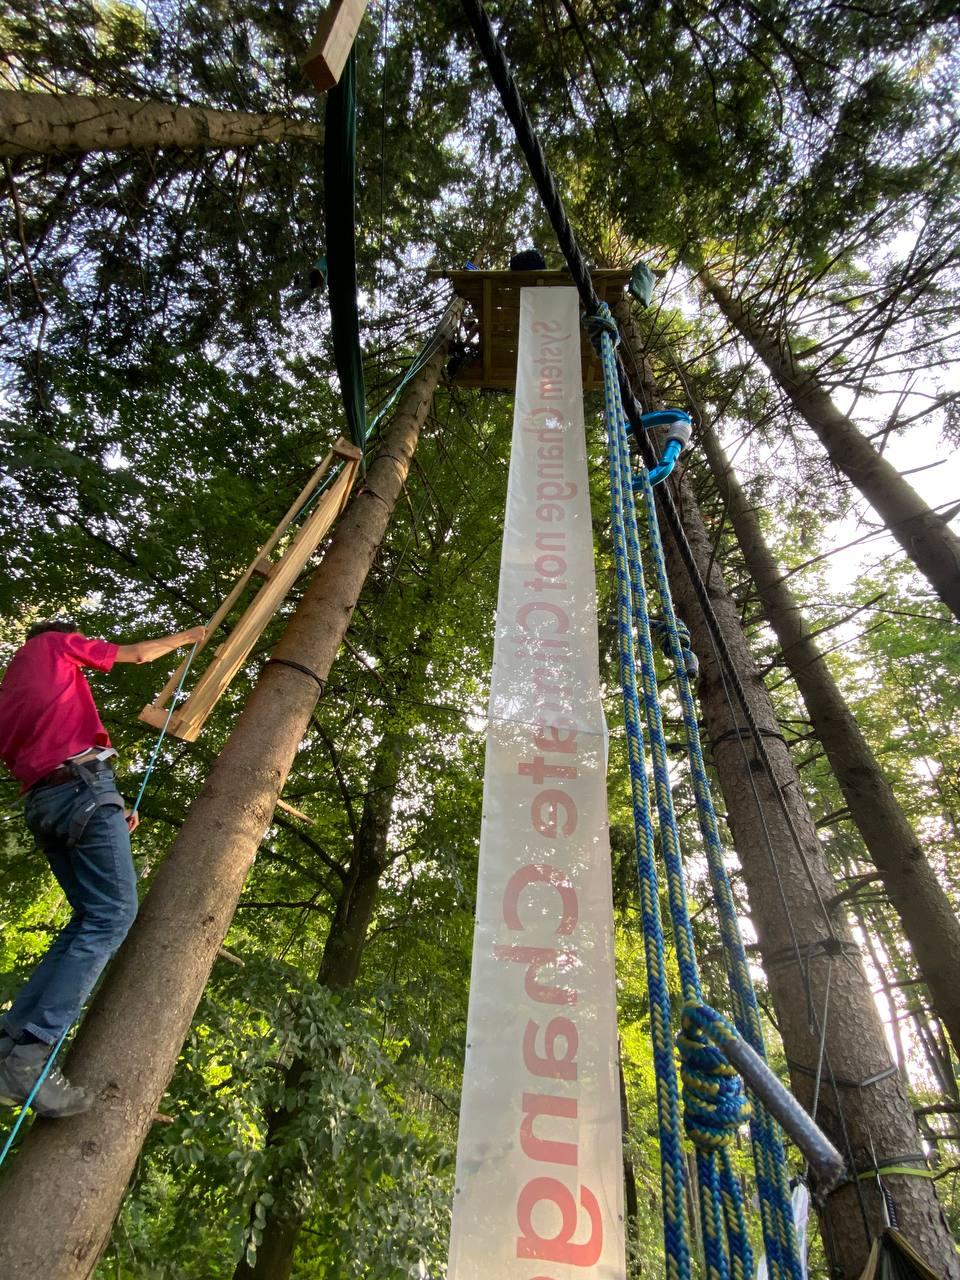
\includegraphics[width=\paperwidth]{forest2}\end{minipage}}
\begin{frame}[c]
  \centering
  \color{white}

  \bigskip
  \bigskip
  \bigskip
  \bigskip
  \bigskip
  \bigskip
  \bigskip
  \bigskip
  \bigskip

  \scriptsize

  \setbeamercolor{block body}{bg=black!100}
  \begin{minipage}{0.52\textwidth}
    \begin{block}{}
      \centering\normalsize\color{white}
      \hil{\color{white}Computing an integer using the \\ modal toposophic multiverse} \\[-0.4em]
      \
    \end{block}
  \end{minipage}

  \bigskip
  \bigskip
  \bigskip
  \bigskip
  \bf
  \colorbox{black}{\begin{minipage}{0.2\textwidth}
    \centering
    Logique à Paris \\
    February 26th, 2025
  \end{minipage}}
  \bigskip

  \colorbox{black}{\begin{minipage}{0.2\textwidth}
    \centering
    Ingo Blechschmidt \\
    University of Antwerp
  \end{minipage}}
\end{frame}}

\definecolor{mypurple}{RGB}{150,0,255}
\setbeamercolor{structure}{fg=mypurple}

{\usebackgroundtemplate{\begin{minipage}{\paperwidth}\vspace*{2.1em}
\includegraphics[height=\paperheight]{sea-of-clouds-1}\end{minipage}}
\begin{frame}{Well quasi-orders}
  \jnote{1}{
    Well quasi-orders are an important notion in proof theory and termination
    analysis.
  }

  \jnote{2-3}{
    The presented proof rests on the law of excluded middle and hence cannot
    immediately be interpreted as a program for finding suitable indices~$i <
    j$. However, constructive proofs are also possible (for instance by
    induction on the value of a given term of the sequence, see
    \href{https://www.math.lmu.de/~petrakis/Dickson.pdf}{Constructive
    combinatorics of Dickson's Lemma} by Iosif Petrakis for several fine
    quantitative results). And even more:
    There is a procedure for regarding this proof---and many others in the
    theory of well quasi-orders---as \emph{blueprints} for more informative
    constructive proofs. This shall be our motto for today:

    \emph{Do not take classical proofs literally, instead ask which
    constructive proofs they are blueprints for.}
  }

  \jnote{3}{
    The displayed stability results, along with several others, provide a
    flexible toolbox for constructing new well quasi-orders from given ones.
    However, with the classical formulation of \emph{well},
    renamed~``well\sinf'' on the next slide, these results are inherently
    classical.

    In Higman's lemma, the set~$X^*$ of finite lists of elements of~$X$ is
    equipped with the following ordering: We have~$x_0 \ldots x_{n-1} \leq y_0
    \ldots y_{m-1}$ iff there is an increasing injection~$f : \{ 0,\ldots,n-1 \} \to \{
    0,\ldots,m-1 \}$ such that~$x_i \leq y_{f(i)}$ for all~$i < n$.
  }

  \jnote{4}{
    \vspace*{-1em}
    The dependence of the theory on well quasi-orders on classical transfinite
    methods is already present in one of the first and central observations of this theory:

    \textbf{Lemma.} Let~$X$ be well\sinf. Let~$\alpha : \NN \to X$. Then there
    is an infinite increasing subsequence~$\alpha\,i_0 \leq \alpha\,i_1 \leq
    \ldots$.

    \emph{Proof.} Let~$K \defeq \{ n \in \NN \,|\, \neg \exists m > n\_
    \alpha\,n \leq \alpha\,m \}$ be the set of indices of those terms which cannot
    appear as the first component of a good pair. If~$K$ is in bijection
    with~$\NN$, there is a subsequence~$\alpha\,k_0 \leq \alpha\,k_1 \leq
    \ldots$ with~$k_0, k_1, \ldots \in K$. As~$X$ is well\sinf, this sequence
    is good, a contradiction.

    Hence~$K$ is not in bijection with~$\NN$. Assuming~\bad{\textsc{lem}},
    it is hence bounded by a number~$N$, and (again
    with~\bad{\textsc{lem}}), for every index~$a > N$ there is an index~$b >
    a$ such that~$\alpha\,a \leq \alpha\,b$. Thus,
    assuming~\bad{\textsc{dc}}, every number~$i_0 > N$ is a suitable
    starting index for an infinite increasing subsequence. \qed

    The appeal to dependent choice can be removed by always picking the
    smallest possible next index in~$\NN \setminus K$, doable by yet another
    invocation of~\bad{\textsc{lem}}. But the result remains fundamentally
    noneffective---in the special case~$X = (\{ 0, 1 \}, {=})$, the statement
    of the lemma implies the infinite pigeonhole principle.
  }

  \jnote{5-7}{
    Luckily, thanks to work by Thierry Coquand, Daniel Fridlender and Monika
    Seisenberger, a constructive substitute is available, the notion well\ind.
    In classical mathematics (where~\textsc{lem} and~\textsc{dc} and hence bar
    induction are available), this notion is equivalent to well\sinf.

    The assertion~``$\mathsf{Good} \mid [\,]$'' is pronounced ``$\mathsf{Good}$
    bars the empty list'', and is defined as follows: Let~$B$ be a predicate
    on~$X^\star$. Then~$B \mid
    \sigma$ is inductively generated by the following two clauses.

    \vspace*{-0.5em}
    \begin{enumerate}
      \item If~$B\sigma$, then~$B \mid \sigma$.
      \\[-1.3em]
      \item If~$B \mid \sigma x$ for all~$x \in X$, then~$B \mid \sigma$.
    \end{enumerate}
    \vspace*{-0.5em}

    Here~$\sigma x$ denotes the concatenation of the list~$\sigma$ with the
    element~$x$. The accompanying induction principle is the following: Let~$Q$
    be a predicate on~$X^*$ such that, for all~$\sigma \in X^*$,~$B\sigma \Rightarrow Q\sigma$ and
    $(\forall x \in X\_ Q(\sigma x)) \Rightarrow Q\sigma$. Then, for
    all~$\sigma \in X^*$: If~$B \mid \sigma$, then~$Q\sigma$.

    Intuitively, the assertion~``$B \mid \sigma$'' expresses (in a positive
    direct way) that no matter how~$\sigma$ evolves to a longer finite
    list~$\tau$, eventually~$B\tau$ will hold.
  }

  \jnote{8}{
    \begin{columns}[t]
      \begin{column}{0.60\textwidth}
        The original notion well\sinf:
        \begin{itemize}
          \justifying
          \item[\cmark] short and simple
          \\[-1.3em]
          \item[\cmark] constructively satisfied for the main examples (but
          only because of the theory around well\ind)
          \\[-1.3em]
          \item[\cmark] concise abstract proofs (albeit employing transfinite methods)
          \\[-1.3em]
          \item[\xmark] main results not constructively attainable
          \\[-1.3em]
          \item[\xmark] philosophically strenuous by the quantification over all sequences
          \\[-1.3em]
          \item[\xmark] not stable under ``change of base''---a forcing extension
          of the universe may well contain more sequences than the base universe
          \\[-1.3em]
          \item[\xmark] negative (universal) condition
        \end{itemize}
      \end{column}

      \begin{column}{0.45\textwidth}
        The constructive substitute well\ind:
        \begin{itemize}
          \justifying
          \item[\cmark] main results constructive
          \\[-1.3em]
          \item[\cmark] stable under change of base
          \\[-1.3em]
          \item[\cmark] positive (existential) condition
          \\[-1.3em]
          \item[\xmark] proofs intriguing, but also somewhat alien, not just some
          trivial reshuffling of the classical arguments, classical sequence
          language cannot be used
        \end{itemize}
      \end{column}
    \end{columns}
  }

  \jnote{9}{
    Constructively, the notion~well\ind is much stronger than~well\sinf, as it
    ensures goodness (in an appropriate sense) of sequence-like entities
    which are not actually honest maps~$\NN \to X$.

    For partial maps~$\alpha$, by~$\alpha\,n\,\downarrow$ we mean that~$\alpha$
    is defined on the input~$n$. If~\bad{\textsc{lem}} is available, then a
    partial map such that~$\neg\neg(\alpha\,n\,\downarrow)$ for all~$n \in \NN$
    is already a total map, but without~\bad{\textsc{lem}} the hypothesis
    well\sinf{} does not have anything to say about such a partially-defined
    sequence.

    If~\bad{\textsc{dc}} is available, then every multivalued map contains a
    singlevalued map, but again without~\bad{\textsc{dc}} the hypothesis well\sinf{}
    does not have anything to say about multivalued sequences.
  }

  \jnote{10}{
    It turns out that these entities are, or give rise to, actual maps~$\NN \to
    X$---but in a forcing extension of the universe.

    Forcing originated in set theory to construct new models for set theory
    from given ones, in order to explore the range of set-theoretic
    possibility. For instance, by forcing we can construct models of~\text{zfc}
    validating the continuum hypothesis and also models which falsify it.

    We here refer to a simplification of original forcing which is useful in a
    constructive metatheory. At its core, every forcing extension is just a
    formula and proof translation of a certain form. For instance, there is a
    forcing extension validating~\bad{\textsc{lem}} even if the base universe
    does not; this forcing extension is not a deep mystery, for a statement holds
    in that forcing extension iff its double negation translation holds in the
    base universe and it is well-known that the double negation translation
    of~\bad{\textsc{lem}} is an intuitionistic tautology.

    \href{https://www.speicherleck.de/iblech/stuff/slides-herrsching2023.pdf}{Here
    is a set of slides on constructive forcing}, and Section~4 of
    \href{https://raw.githubusercontent.com/iblech/constructive-maximal-ideals/master/tex/extended.pdf}{this
    joint paper with Peter Schuster} contains a written summary of constructive
    forcing.
  }

  \textbf{Def.} Let~$(X,{\leq})$ be a quasi-order.
  \vspace*{-0.3em}
  \begin{itemize}
    \item A sequence~$\alpha : \NN \to X$ is \hil{good} iff
    there exist~$i < j$ with~$\alpha\,i \leq \alpha\,j$.
    \item The quasi-order~$X$ is \hil{well\only<4->{\sinf}} iff every sequence~$\NN \to X$ is good.
  \end{itemize}
  \pause
  \vspace*{-0.9em}

  \begin{columns}[t]
    \begin{column}{0.46\textwidth}
      \begin{block}{Natural numbers\phantom{y}}
        \textbf{Prop.} $(\NN, {\leq})$ is well\only<4->{\sinf}.
        \smallskip

        \emph{Proof.} Let~$\alpha : \NN \to \NN$. By~\badbox{\textsc{lem}}, there is a
        \bad{minimum}~$\alpha\,i$.
        Set~$j \defeq i + 1$. \qed

        \hfill\color{gray}offensive?
      \end{block}
      \only<2-4>{
        \vspace*{-2em}
        \[ \astikznodetransparentlycircled{xm}{7}\!,
        \quad \astikznodetransparentlycircled{x0}{4}\!,
        \quad \astikznodecircled{t1}{mypurple}{3}\!,
        \quad \astikznodetransparentlycircled{x1}{1}\!,
        \quad \astikznodecircled{t2}{mypurple}{8}\!,
        \quad \astikznodetransparentlycircled{x2}{2}\!,
        \quad \ldots \]
      {\centering\begin{tikzpicture}[remember picture,overlay]
        \node[draw=mypurple, circle, thick, inner sep=0.1em] (t3) {\scriptsize$\leq$};
        \path[draw=mypurple,thick]
          (t1)
          to [out=-90, in=180] (t3)
          to [out=0, in=-90] (t2);
      \end{tikzpicture}\par}}
    \end{column}

    \pause

    \begin{column}{0.50\textwidth}
      \begin{block}{Key stability results}
        \justifying
        \only<1-5>{Assuming~\badbox{\textsc{lem}}
        and~\badbox{\textsc{dc}}}\only<6->{\good{Constructively}}, \ldots

        \hil{Dickson:} \tabto{1.8cm} If~$X$ and~$Y$ are well\only<4-5>{\sinf}\only<6->{\ind}, so is~$X \times Y$. \\
        \hil{Higman:}  \tabto{1.8cm} If~$X$ is well\only<4-5>{\sinf}\only<6->{\ind}, so is~$X^\star$. \\
        \hil{Kruskal:} \tabto{1.8cm} If~$X$ is well\only<4-5>{\sinf}\only<6->{\ind}, so is~$\mathrm{Tree}(X)$.
      \end{block}
    \end{column}
  \end{columns}
  \pause
  \pause

  \textbf{Def.} A quasi-order~$X$ is \hil{well\ind} iff there exists a
  \hil{modulus of wellness} for~$X$.
  \pause
  \pause

  \small
  With \bad{bar induction},\tabto{3.10cm} $\text{well}\ind \Leftarrow \text{well}\sinf$. \\[-0.2em]
  Constructively,\tabto{3.10cm} $\text{well}\ind \Rightarrow \text{well}\sinf$.
  \only<8>{
    \bigskip
    \begin{columns}[c]
      \begin{column}{0.01\textwidth}
	
\includegraphics[height=2.4em]{question-mark}
      \end{column}
      \begin{column}{0.9\textwidth}
      Is there a procedure for reinterpreting \hil{classical proofs}
      regarding well\sinf{} as \newline \hil{blueprints for constructive proofs} regarding well\ind?
      \end{column}
    \end{columns}
  }
  \pause
  \pause
  Moreover, if~$X$ is well\ind, then \ldots
  \begin{itemize}
  \vspace*{-0.7em}
    \small
    \item for every \emph{partial} function~$\alpha$,\tabto{5.25cm}
    if~$\forall n\_ \neg\neg(\alpha\,n\,{\downarrow})$,
    then~$\neg\neg \exists i < j\_ \alpha\,i\,{\downarrow} \wedge
    \alpha\,j\,{\downarrow} \wedge \alpha\,i \leq \alpha\,j$. \\[-2.0em]\
    \item for every \emph{multivalued} function~$\alpha$,\tabto{5.25cm}
    $\exists i < j\_ \exists x \in \alpha\,i\_
    \exists y \in \alpha\,j\_ x \leq y$.
  \end{itemize}
  \pause

  \vspace*{-0.7em}
  \hil{Central insight:} A quasi-order $X$ is well\ind iff $\hil{$\necessary$}\,\forall\alpha : \NN \to
  X\_ \exists i < j\_ \alpha\,i \leq \alpha\,j$.
\end{frame}}

{\usebackgroundtemplate{\begin{minipage}{\paperwidth}\vspace*{0.29cm}\hspace*{-1cm}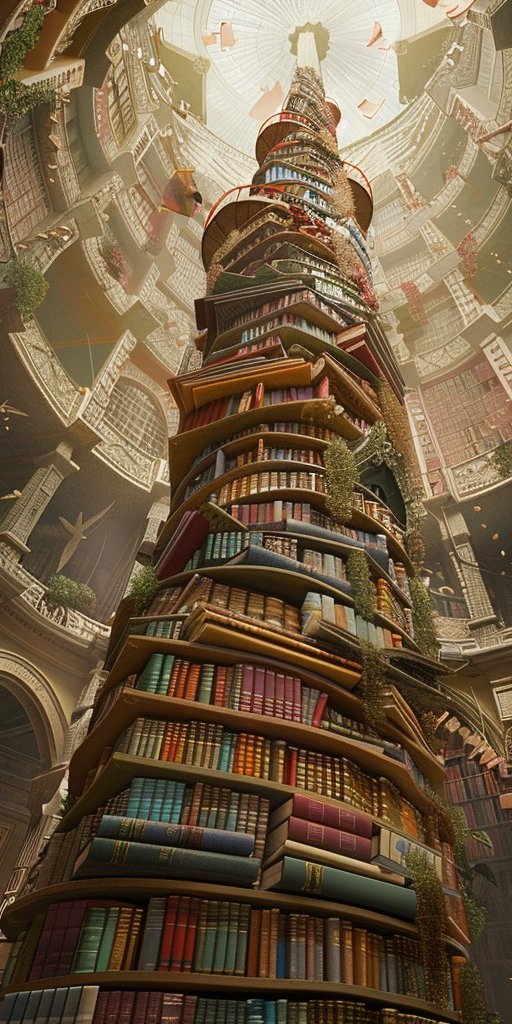
\includegraphics[height=\paperheight]{tower-cropped}\end{minipage}}
\begin{frame}{The modal multiverse of constructive forcing}
  \jnote{1}{
    By \emph{topos}, we mean \emph{Grothendieck topos}. In constructive
    forcing, a ``forcing extension of the base universe'' is exactly the same
    thing as a Grothendieck topos.

    A particular member of the rich and varied landscape of toposes is the
    \emph{trivial topos}, in which every statement whatsoever holds. By
    restricting to positive toposes, we exclude this special case.

    For positive toposes~$\E$, a geometric implication holds in~$\E$ iff it
    holds in the base universe. For positive overt toposes~$\E$, we even have
    that a bounded first-order formula holds in~$\E$ iff it holds in the base.
    Hence, for the purpose of verifying a bounded first-order assertion about
    the base, we can freely pass to a positive overt topos with problem-adapted
    better higher-order properties (such as that some uncountable set from the
    base now appears countable, or that an infinite sequence whose existence is
    predicted by failing dependent choice now actually exists).

    \href{https://www.speicherleck.de/iblech/stuff/early-draft-modal-multiverse.pdf}{Here
    is a rough early draft of a preprint with more details about the modal
    multiverse.}
  }

  \jnote{2}{
    The idea to study the modal multiverse of toposes in a principled manner
    was proposed by Alexander Oldenziel in 2016. \emph{Foreshadowed by:}
    \begin{itemize}
      \item[1984\phantom{s}] André Joyal, Miles Tierney. ``An extension of the Galois theory of Grothendieck''.
      \\[-1em]
      \item[1987\phantom{s}] Andreas Blass. ``Well-ordering and induction in intuitionistic logic and topoi''.
      \\[-1em]
      \item[2010s] Milly Maietti, Steve Vickers. Ongoing work on arithmetic universes.
      \\[-1em]
      \item[2011\phantom{s}] Joel David Hamkins. ``The set-theoretic multiverse''.
      \\[-1em]
      \item[2013\phantom{s}] Shawn Henry. ``Classifying topoi and preservation of higher order logic by geometric morphisms''.
    \end{itemize}
  }

  \jnote{3}{
    With the modal language we seek to provide an accessible and modular
    framework for constructivization results.

    For instance, conservativity of classical logic over intuitionistic logic
    for geometric implications (known under various names such as Barr's
    theorem, Friedman's trick, escaping the continuation monad, \ldots) is
    packaged up by the observation that \emph{somewhere}, the law of excluded
    middle holds.

    Another example:
    In the community around Krull's lemma, it is well-known that
    we can constructively infer that a given ring element~$x \in A$ is nilpotent from
    knowing that it is contained in the \emph{generic prime ideal} of~$A$. This entity
    is not actually an honest prime ideal of the ring~$A$ in the base
    universe, but a certain combinatorial notion (efficiently dealt with using
    \emph{entailment relations}). Constructive forcing allows us to reify the
    generic prime ideal as an actual prime ideal in a suitable forcing extension,
    so in a suitable topos (der little Zariski topos of the ring).
  }

  \begin{changemargin}{7.5em}{-0.5em}
    \textbf{Def.} A statement~$\varphi$ holds \ldots
    \vspace*{-0.3em}
    \begin{itemize}
      \small
      \item \hil{everywhere} \tabto{2.15cm}($\necessary\varphi$)\tabto{3.08cm}
      iff it holds \hil{in every topos}
      (over the current base).
      \item \hil{somewhere} \tabto{2.15cm}($\possible\varphi$)\tabto{3.08cm} iff
      it holds \hil{in some positive topos}.
      \item \hil{proximally} \tabto{2.15cm}($\xpossible\varphi$)\tabto{3.08cm}
      iff it holds \hil{in some positive overt topos}.
    \end{itemize}

    \textbf{Def.} A (Grothendieck) \hil{topos} is a category equivalent to the
    category of sheaves over a small site.
    \pause

    \only<2>{
      \textbf{Examples for toposes.}
      \begin{itemize}
        \item $\mathrm{Set}$, the category of sets and maps.
        \item The category of sets and maps which are \hil{defined up to~$\boldsymbol{\neg\neg}$}.
        \item $\mathrm{Set}[G]$, the extension obtained by adding a \hil{generic
        filter} of a \hil{forcing notion} (a quasi-order equipped with a
        coverage).
      \end{itemize}
      The following are \bad{not} toposes:
      \begin{itemize}
        \item The category of sets and partially defined maps.
        \item The category of abelian groups.
      \end{itemize}
    }

    \visible<3->{
      \hil{Multiversal yoga:}
      \begin{enumerate}
        \item A quasiorder is well\ind iff \emph{everywhere}, every sequence is good.
        \smallskip
        \item A ring element is nilpotent iff \\ all prime ideals \emph{everywhere} contain it.
        \smallskip
        \item For every inhabited set~$X$, \\ \emph{proximally} there exists an
        enumeration~$\NN \twoheadrightarrow X$.
        \smallskip

        \item For every ring, \emph{proximally} there exists a maximal ideal.
        \smallskip

        \item \emph{Somewhere}, the law of excluded middle holds.
      \end{enumerate}
    }
  \end{changemargin}
\end{frame}}

{\usebackgroundtemplate{\begin{minipage}{\paperwidth}\vspace*{-4.68em}
\includegraphics[width=1.2\paperwidth]{wqo-faded}\end{minipage}}
\begin{frame}{Multiversal constructive combinatorics}
  \jnote{1}{
    The displayed multiversal proof closely mimics the classical proof (for well\sinf), but
    is fully constructive (for well\ind). It would be possible to streamline
    this proof and unroll the topos-theoretic machinery, to obtain an explicit
    algorithm of type
    \[ \mathsf{Good} \mid_X [\,] \times \mathsf{Good} \mid_Y [\,] \ \longrightarrow\
      \mathsf{Good} \mid_{X \times Y} [\,].
    \]

    The modal language was recently used to answer a question by Stefano
    Berardi, Gabriele Buriola and Peter Schuster, see
    \href{https://www.speicherleck.de/iblech/stuff/slides-abmv2024.pdf\#page=16}{this
    set of slides}.
  }

  \justifying
  \textbf{Prop.} Let~$X$ and~$Y$ be well\ind quasi-orders. Then~$X \times Y$
  is well$\ind$.

  \emph{Multiversal constructive proof.} Let~$\alpha = (\beta,\gamma) : \NN \to X \times Y$ be a sequence in an
  arbitrary topos. We need to show that~$\alpha$ is good, i.\,e.\@ find indices~$n < m$ such that
  \[ \beta\,n \leq \beta\,m \quad\text{and}\quad \gamma\,n \leq \gamma\,m. \]

  It suffices to prove that \emph{somewhere}, $\alpha$ is good, as goodness is
  a geometric implication (in fact even a geometric formula). Hence without loss of
  generality, we may suppose~\textsc{lem}.

  Thus there is an infinite increasing subsequence
  \[ \beta\,k_0 \leq \beta\,k_1 \leq \ldots. \]
  As~$Y$ is well\ind, the sequence~$(\gamma\,k_0, \gamma\,k_1, \ldots)$
  is good, so there exist~$i < j$ with~$\gamma\,k_i \leq \gamma\,k_j$. Since we
  also have~$\beta\,k_i \leq \beta\,k_j$, we are done. \qed
\end{frame}}

{\usebackgroundtemplate{\begin{minipage}{\paperwidth}\vspace*{5.95cm}
\includegraphics[width=\paperwidth]{fr1}\end{minipage}}
\begin{frame}{Multiversal constructive algebra}
  \jnote{1-}{
    The displayed classical proof is quite efficient from the point of view of
    organizing mathematical knowledge, as it quickly reduces the general
    situation of dealing with an arbitrary ring to dealing with a field.
    Alas, read literally, it is hopeless ineffective.
  }

  \jnote{2-}{
    By employing modal language, we can closely mimic the original proof and be
    fully constructive at the same time.
  }

  \jnote{3-}{
    By unwinding all modal definitions, the modal proof can be unrolled to a
    fully explicit computation.
  }

  \justifying
  \textbf{Thm.}
  Let~$M$ be a surjective matrix with more rows than columns over a
  ring~$A$. Then~$1 = 0$ in~$A$.
  \medskip

  \emph{Classical proof.}
  \bad{Assume not.} Then there is~a \bad{maximal ideal} $\mmm$.
  The matrix~$M$ is surjective over~$A/\mmm$. Since~$A/\mmm$ is a field, this
  is a contradiction to basic linear algebra. \qed
  \medskip
  \pause

  \emph{Multiversal constructive proof.}
  We may work \emph{somewhere} where \good{\textsc{lem}} holds. So \good{assume not}.
  \emph{Proximally,} there is a \good{maximal ideal}~$\mmm$.
  The matrix~$M$ is still surjective \emph{there}, and also over~$A/\mmm$. Since~$A/\mmm$ is a field, this
  is a contradiction to basic linear algebra. \qed
  \medskip
  \pause

  \emph{Unrolled constructive proof (special case).}
  Write~$M =
  \left(\begin{smallmatrix}x\\y\end{smallmatrix}\right)$. By surjectivity,
  have~$u, v$ with
  \vspace*{-0.6em}
  \[
    u \left(\begin{smallmatrix}x\\y\end{smallmatrix}\right) = \left(\begin{smallmatrix}1\\0\end{smallmatrix}\right)
    \quad\text{and}\quad
    v \left(\begin{smallmatrix}x\\y\end{smallmatrix}\right) = \left(\begin{smallmatrix}0\\1\end{smallmatrix}\right).
  \]
  Hence
  $
    1 = (vy) (ux) = (uy) (vx) = 0
  $.
  \qed
  \pause

  \centering
  \emph{\href{https://iblech.github.io/constructive-maximal-ideals/}{Agda
  formalization available.}}
  \par
\end{frame}}


\backupstart

\begin{frame}
  \emph{Backup slides.}
\end{frame}

\section{Basics of forcing}

\begin{frame}{Ingredients for forcing}
  \vspace*{-0.3em}
  To construct a forcing extension, we require:
  \begin{enumerate}
    \item a base universe~$V$
    \item a preorder~$L$ of \hil{forcing conditions} in~$V$\!,
    pictured as \hil{finite approximations}

    (\emph{convention:} $\tau \preccurlyeq \sigma$ means that~$\tau$ is a
    better finite approximation than~$\sigma$)
    \item a \hil{covering system} governing how finite approximations evolve to
    better ones

    (for each~$\sigma \in L$, a set~$\Cov(\sigma) \subseteq
    P({\downarrow}\sigma)$, with a simulation condition)
  \end{enumerate}
  In the forcing extension~$V^\nabla$, there will then be a \hil{generic filter} (ideal
  object).
  \pause

  \vspace*{-1em}
  \begin{columns}
    \begin{column}{0.49\textwidth}
      \small
      \begin{block}{For the generic surjection~$\NN \twoheadrightarrow X$}
        \justifying
        Use \hil{finite lists}~$\sigma \in X^*$ as forcing conditions,
        where $\tau \preccurlyeq \sigma$ iff~$\sigma$ is an initial segment of~$\tau$,
        and be prepared to grow~$\sigma$ to \ldots
        \footnotesize
        \begin{enumerate}
          \item[(a)] one of~$\{ \sigma x \,|\, x \in X \}$, to make~$\sigma$ more defined
          \item[(b)] one of~$\{ \sigma \tau \,|\, \tau \in X^*, a \in
          \sigma\tau \}$, for any~$a \in X$, to make~$\sigma$ more surjective
        \end{enumerate}
        \vspace*{-0.4em}
      \end{block}
    \end{column}
    \pause

    \begin{column}{0.45\textwidth}
      \small
      \begin{block}{For the generic prime ideal of a ring~$A$}
        \justifying
        Use \hil{f.g.\@ ideals} as forcing conditions, where $\bbb \preccurlyeq
        \aaa$ iff~$\bbb \supseteq \aaa$, and be prepared to grow~$\aaa$ to \ldots
        \footnotesize
        \begin{enumerate}
          \item[(a)] one of~$\emptyset$, if~$1 \in \aaa$, to make~$\aaa$ more proper
          \item[(b)] one of~$\{ \aaa+(x), \aaa+(y) \}$, if~$xy \in \aaa$, to
          make~$\aaa$ more prime
        \end{enumerate}
        \vspace*{-0.4em}
      \end{block}
    \end{column}
  \end{columns}
\end{frame}

{\usebackgroundtemplate{\begin{minipage}{\paperwidth}\vspace*{-1cm}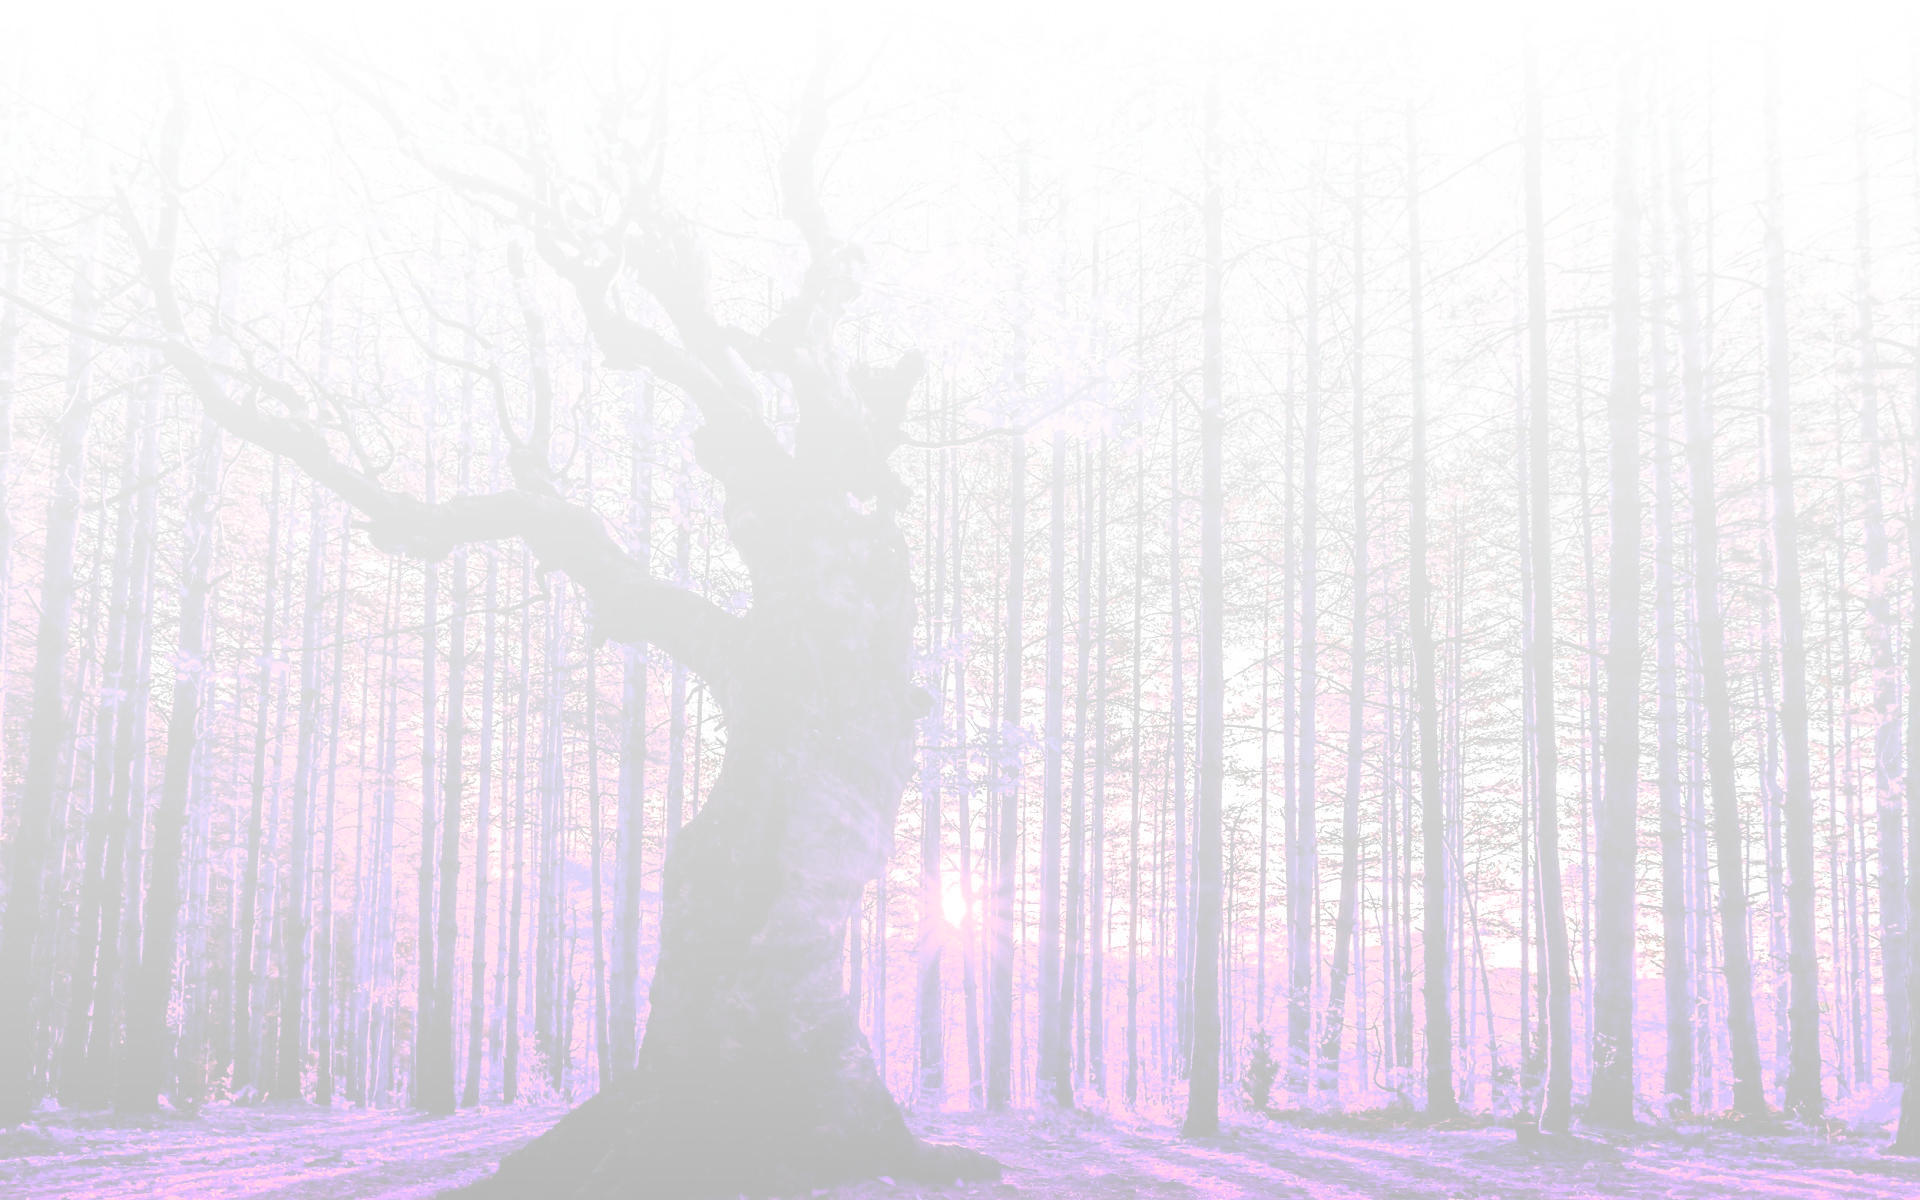
\includegraphics[width=\paperwidth]{forest-light-colored}\end{minipage}}
\begin{frame}{The eventually monad}
  Let~$L$ be a forcing notion.

  Let~$P$ be a monotone predicate on~$L$
  (if $\tau \preccurlyeq \sigma$, then $P\sigma \Rightarrow P\tau$). \\
  For instance, in the case~$L = X^*$:
  \begin{itemize}
    \item $\mathsf{Repeats}\, x_0\ldots x_{n-1} \defeqv \exists i\_ \exists j\_ i < j \wedge x_i = x_j$
    \item $\mathsf{Good}\, \,\,\,\,\,\,x_0\ldots x_{n-1} \defeqv \exists i\_ \exists j\_ i < j \wedge x_i \leq x_j$
    \quad (for some preorder~$\leq$ on~$X$)
  \end{itemize}
  \pause

  We then define~``\hil{$P \mid \sigma$}'' (``$P$ bars~$\sigma$'') inductively by the following clauses:
  \begin{enumerate}
    \item If~$P\sigma$, then~$P \mid \sigma$.
    \item If~$P \mid \tau$ for all~$\tau \in R$, where~$R$ is some covering
    of~$\sigma$, then~$P \mid \sigma$.
  \end{enumerate}
  So~$P \mid \sigma$ expresses in a \hil{direct inductive fashion}:
  \[ \text{``No matter
  how~$\sigma$ evolves to a better approximation~$\tau$, eventually~$P\tau$
  will hold.''} \]

  \pause
  We use quantifier-like notation: ``$\nabla(\tau \preccurlyeq \sigma)\_
  P\tau$'' means ``$P \mid \sigma$''.
\end{frame}}
% BOARD:
% - examples for P | σ
% - abuse of notation

\begin{frame}{Proof translations}
  \textbf{Thm.} Every~\textsc{iqc}-proof remains correct, with at most a
  polynomial increase in length, if throughout we
  replace
  \[\begin{array}{rcl@{\quad\text{where}\quad}rcl}
    \exists & \leadsto & \exists^\mathrm{cl},
    & \exists^\mathrm{cl} &\defeqv& \neg\neg\exists, \\
    \vee & \leadsto & \vee^\mathrm{cl},
    & \alpha \vee^\mathrm{cl} \beta &\defeqv& \neg\neg(\alpha \vee \beta), \\
    = & \leadsto & =^\mathrm{cl},
    & s =^\mathrm{cl} t &\defeqv& \neg\neg(s = t).
  \end{array} \]
  \pause

  \begin{columns}[c]
    \begin{column}{0.01\textwidth}
      
\includegraphics[height=2.4em]{sheafification-man-2}
    \end{column}
    \quad
    \begin{column}{0.9\textwidth}
      \hil{When we say:}\ \ some statement ``holds in~$V^{\neg\neg}$'', \\
      \makesamewidth[l]{\hil{When we say:}}{\hil{we mean:}}\ \ its translation holds in~$V$.
    \end{column}
  \end{columns}
  \bigskip

  Similarly for arbitrary forcing extensions~$V^\nabla$, ``just with~$\nabla$
  instead of~$\neg\neg$''.
  \bigskip

  \pause
  \textbf{Ex.} As~$\neg\neg(\varphi \vee \neg\varphi)$ is a theorem
  of~\textsc{iqc}, the law of excluded middle holds in~$V^{\neg\neg}$.
\end{frame}

\newcommand{\defeqvi}{\quad iff\quad}
\begin{frame}{The $\nabla$-translation}
  \small
  \only<1>{For bounded first-order formulas over the (large) first-order signature which has
  \begin{enumerate}
    \scriptsize
    \item one sort~$\underline{X}$ for each set~$X$ in the base universe,
    \\[-1.2em]
    \item one~$n$-ary function symbol~$\underline{f} : \underline{X_1} \times
    \cdots \times \underline{X_n} \to \underline{Y}$ for each map~$f : X_1 \times
    \cdots \times X_n \to Y$,
    \\[-1.2em]
    \item one~$n$-ary relation symbol~$\underline{R} \hookrightarrow
    \underline{X_1} \times \cdots \times \underline{X_n}$ for each relation~$R
    \subseteq X_1 \times \cdots \times X_n$, and
    \\[-1.2em]
    \item an additional unary relation symbol~$G \hookrightarrow \underline{L}$
    (for the \emph{generic filter} of~$L$),
  \end{enumerate}
  we recursively define:}
  \scriptsize
  \only<2->{\vspace*{-0.4em}}
  \begin{tabbing}
    \quad \= $\sigma \forces \forces \forall(x\?\underline{X})\_ \varphi$ \=
    \defeqvi $\textcolor{gray}{\forall(\tau \preccurlyeq \sigma)\_}\
    \forall(x_0 \in X)\_ \tau \forces \varphi[\underline{x_0}/x]$.\qquad\quad \=
    $\sigma \forces \exists(x\?\underline{X})\_ \varphi$
    \= $\sigma \forces \underline{R}(\underline{s_1},\ldots,\underline{s_n})$ \= \defeqvi $s = t$. \= \kill

    \> $\sigma \forces s = t$
    \> \defeqvi $\nabla \sigma\_ \llbracket s \rrbracket = \llbracket t \rrbracket$.
    \> $\sigma \forces \underline{R}(s_1,\ldots,s_n)$
    \> \defeqvi $\nabla\sigma\_ R(\llbracket s_1 \rrbracket,\ldots,\llbracket s_n \rrbracket)$. \\[0.3em]

    \> $\sigma \forces \varphi \Rightarrow \psi$
    \> \defeqvi $\textcolor{gray}{\forall(\tau \preccurlyeq \sigma)\_}\ (\tau \forces \varphi) \Rightarrow
    (\tau \forces \psi)$.
    \> $\sigma \forces G\tau$
    \> \defeqvi $\nabla\sigma\_ \sigma \preccurlyeq \llbracket\tau\rrbracket$. \\[0.3em]

    \> $\sigma \forces \top$ \> \defeqvi $\top$.
    \> $\sigma \forces \bot$ \> \defeqvi $\hil{$\nabla\sigma\_$}\ \bot$ \\[0.3em]

    \> $\sigma \forces \varphi \wedge \psi$
    \> \defeqvi $(\sigma \forces \varphi) \wedge (\sigma \forces \psi)$.
    \> $\sigma \forces \varphi \vee \psi$
    \> \defeqvi $\hil{$\nabla\sigma\_$}\ (\sigma \forces \varphi) \vee (\sigma \forces \psi)$. \\[0.3em]

    \> $\sigma \forces \forall(x\?\underline{X})\_ \varphi$
    \> \defeqvi $\textcolor{gray}{\forall(\tau \preccurlyeq \sigma)\_}\ \forall(x_0 \in X)\_ \tau \forces
    \varphi[\underline{x_0}/x]$.
    \> $\sigma \forces \exists(x\?\underline{X})\_ \varphi$
    \> \defeqvi $\hil{$\nabla\sigma\_$}\ \exists(x_0 \in X)\_ \sigma \forces \varphi[\underline{x_0}/x]$.
  \end{tabbing}
  \small
  \only<1>{Finally, we say that~$\varphi$ ``holds in~$V^\nabla$'' iff for all~$\sigma
  \in L$, $\sigma \forces \varphi$.}

  \footnotesize
  \begin{tabular}{@{}lp{0.27\textwidth}p{0.48\textwidth}@{}}
    \toprule
    forcing notion & statement about~$V^\nabla$ & external meaning \\
    \midrule
    surjection $\NN \twoheadrightarrow X$ &
    ``the gen.\@ surj.\@ is surjective'' &
    $\forall(\sigma{\in}X^*)\_ \forall(a{\in}X)\_ \nabla(\tau{\preccurlyeq}\sigma)\_ \exists(n{\in}\NN)\_ \tau[n] = a$. \\[0.4em]
    \pause

    map $\NN \to X$ &
    ``the gen.\@ sequence is good'' &
    $\mathsf{Good} \mid [\,]$. \\[0.4em]

    frame of opens &
    ``every complex number has a square root'' &
    For every open~$U \subseteq X$ and every cont.\@
    function $f : U \to \CC$, there is an open covering $U = \bigcup_i U_i$ such
    that for each index~$i$, there is a cont.\@ function $g : U_i \to \CC$
    such that~$g^2 = f$. \\[4.3em]

    big Zariski &
    ``$x \neq 0 \Rightarrow \text{$x$ inv.}$'' &
    If the only f.p.\@ $k$-algebra in which~$x = 0$ is the zero algebra,
    then~$x$ is invertible in~$k$.\\[1.5em]
    \pause

    little Zariski &
    ``every f.g. vector space does \emph{not not} have a basis'' &
    \makesamewidth[l]{}{\phantom{x}}\hil{Grothendieck's generic freeness lemma}
  \end{tabular}
\end{frame}

\begin{frame}{Outlook}
  \begin{block}{Passing to and from extensions}
    \justifying\small
    \textbf{Thm.} Let~$\varphi$ be a \hil{bounded first-order formula} not
    mentioning~$G$. In each of the following situations, we have that
    $\varphi$ holds in~$V^\nabla$ iff~$\varphi$
    holds in $V$:

    \vspace*{-0.5em}
    \begin{enumerate}
      \item $L$ and all coverings are inhabited (proximality). \\[-1em]
      \item $L$ contains a top element, every covering of the
      top element is inhabited, and~$\varphi$ is a coherent implication
      (positivity).
    \end{enumerate}
    \vspace*{-0.8em}
  \end{block}

  \vspace*{-1.5em}
  \begin{columns}
    \begin{column}{0.46\textwidth}
      \begin{block}{The mystery of nongeometric sequents}
        \justifying
        The \hil{generic ideal} of a ring is maximal:
        \vspace*{-1em}
        \[ (x \in \aaa \Rightarrow 1 \in \aaa) \Longrightarrow 1 \in \aaa + (x). \]

        The \hil{generic ring} is a field:
        \vspace*{-0.7em}
        \[ (x = 0 \Rightarrow 1 = 0) \Longrightarrow (\exists y\_ xy = 1). \]
        \vspace*{-1.4em}
      \end{block}

    \end{column}

    \begin{column}{0.50\textwidth}
      \begin{block}{Traveling the multiverse \ldots}
        \textsc{lem} is a \hil{switch} and \hil{holds positively};
        being countable is a \hil{button}.
        \medskip

        Every instance of \textsc{dc} \hil{holds proximally}.
        \medskip

        A geometric implication is provable iff it holds \hil{everywhere}.
        \vspace*{-0.2em}
      \end{block}
      \vspace*{-0.3em}
      \hfill\footnotesize\ldots{} upwards, but always keeping ties to the
      base.{\ }
    \end{column}
  \end{columns}
\end{frame}

\begin{frame}{More on forcing notions}
  \small
  \textbf{Def.} A \hil{forcing notion} consists of
  a preorder~$L$ of \hil{forcing conditions}, and
  for every~$\sigma \in L$, a set~$\Cov(\sigma) \subseteq
  P({\downarrow}\sigma)$ of \hil{coverings} of~$\sigma$
  such that: If~$\tau \preccurlyeq \sigma$ and~$R \in \Cov(\sigma)$, there
  should be a covering~$S \in \Cov(\tau)$ such that~$S \subseteq
  {\downarrow}R$.
  \bigskip

  {\centering\footnotesize\begin{tabular}{llll}
    \toprule
    & preorder~$L$ & coverings of an element~$\sigma \in L$ & filters of~$L$ \\
    \midrule
    \normalnumber{1} & $X^*$ & $\{ \sigma x \,|\, x \in X \}$ & maps~$\NN \to X$ \\
    \normalnumber{2} & $X^*$ & $\{ \sigma x \,|\, x \in X \}$,\ \ $\{ \sigma\tau \,|\, \tau \in X^*, a \in \sigma\tau \}$ for each~$a \in X$ & surjections~$\NN \twoheadrightarrow X$ \\
    \normalnumber{3} & f.g. ideals & --- & ideals \\
    \normalnumber{4} & f.g. ideals & $\{ \sigma+(a), \sigma+(b) \}$ for each~$ab \in \sigma$,\ \ $\{\}$ if~$1 \in \sigma$ & prime ideals \\
    \normalnumber{5} & opens & $\mathcal{U}$ such that~$\sigma = \bigcup \mathcal{U}$ & points \\
    \normalnumber{6} & $\{\star\}$ & $\{ \star \,|\, \varphi \} \cup \{ \star \,|\, \neg\varphi \}$ &
    witnesses of~\textsc{lem}
    \\
    \bottomrule
  \end{tabular}\par}
  \bigskip

  \textbf{Def.} A \emph{filter} of a forcing notion~$(L,\mathrm{Cov})$
  is a subset~$F \subseteq L$ such that
  \vspace*{-0.4em}
  \begin{enumerate}
    \scriptsize
    \item $F$ is upward-closed: if~$\tau \preccurlyeq \sigma$ and if~$\tau \in F$, then~$\sigma \in F$; \\[-3.0em]
    \item $F$ is downward-directed: $F$ is inhabited, and if~$\alpha,\beta \in F$,
    then there is a common refinement~$\sigma \preccurlyeq \alpha,\beta$ such
    that~$\sigma \in F$; and \\[-2.0em]
    \item $F$ splits the covering system: if~$\sigma \in F$ and~$R \in
    \Cov(\sigma)$, then~$\tau \in F$ for some~$\tau \in R$.
  \end{enumerate}
\end{frame}

\backupend

\end{document}

- Well quasi-orders
  *abstract proofs as blueprints for concrete computations?*
  - def. good, well
  - ex. ℕ
  - classical stability results

- A better notion
  - partially defined sequences
    (not really a morphism in Set, but in Sh_¬¬(Set))
  - multivalued sequences
    (approximately morphisms in some category)
  - modulus of wellness

- The modal toposophic multiverse
  - examples for toposes:
    - Set
    - Sh_¬¬(Set)
    - Set[G], obtained by adding a generic filter of a forcing notion
    - not quite toposes: arbitrary partially defined maps, abelian groups
  - modal operators
  - Diamond φ ⇒ φ etc.
  - X has a modulus of wellness iff everywhere, every sequence is good
  - Diamond (¬LEM)
  - etc.

- Applications
  - Dickson, constructively
  - surjective matrices (with Agda)

Somewhere: eigenvalues etc.
